\section{Kurzbeschreibung}
Diese Anleitung dient dem Aufbau sowie dem Einsatz eines einfachen Roboters in einem KURSKURSKURS. Bei diesem Roboter werden zwei Motoren mithilfe eines \textsc{Raspberry-Pi}-Einplatinencomputers angesteuert, um einen Stift über ein  Papierblatt zu bewegen. Die Geschwindigkeit beider Motoren kann dabei durch einfache Programmierbefehle eingestellt werden.\\

Die ursprüngliche Idee des Projektes stammt \href{https://tuduu.org/projekt/automatischer-malroboter}{hierher}\footnote[1]{https://tuduu.org/projekt/automatischer-malroboter}. Da kein \textsc{Calliope} im Filbüro vorhanden war, wurde dieses Projekt auf einem \textsc{Raspberry Pi} umgesetzt, was einige Zwischenschritte erforderte.\\

\subsection{Ziel}
Das Projekt soll den Kursteilnehmern die Möglichkeiten der Programmierung einfacher Elektronik nahebringen.

\section{Vorbereitung}
Je nach Durchführung sowie verfügbarer Zeit sollten einige Schritte des Aufbaus im Vornherein erledigt werden, z.B. die Verdrahtung der Motoren (später beschrieben).\\

\begin{figure}[h]
\centering
\parbox{5cm}{
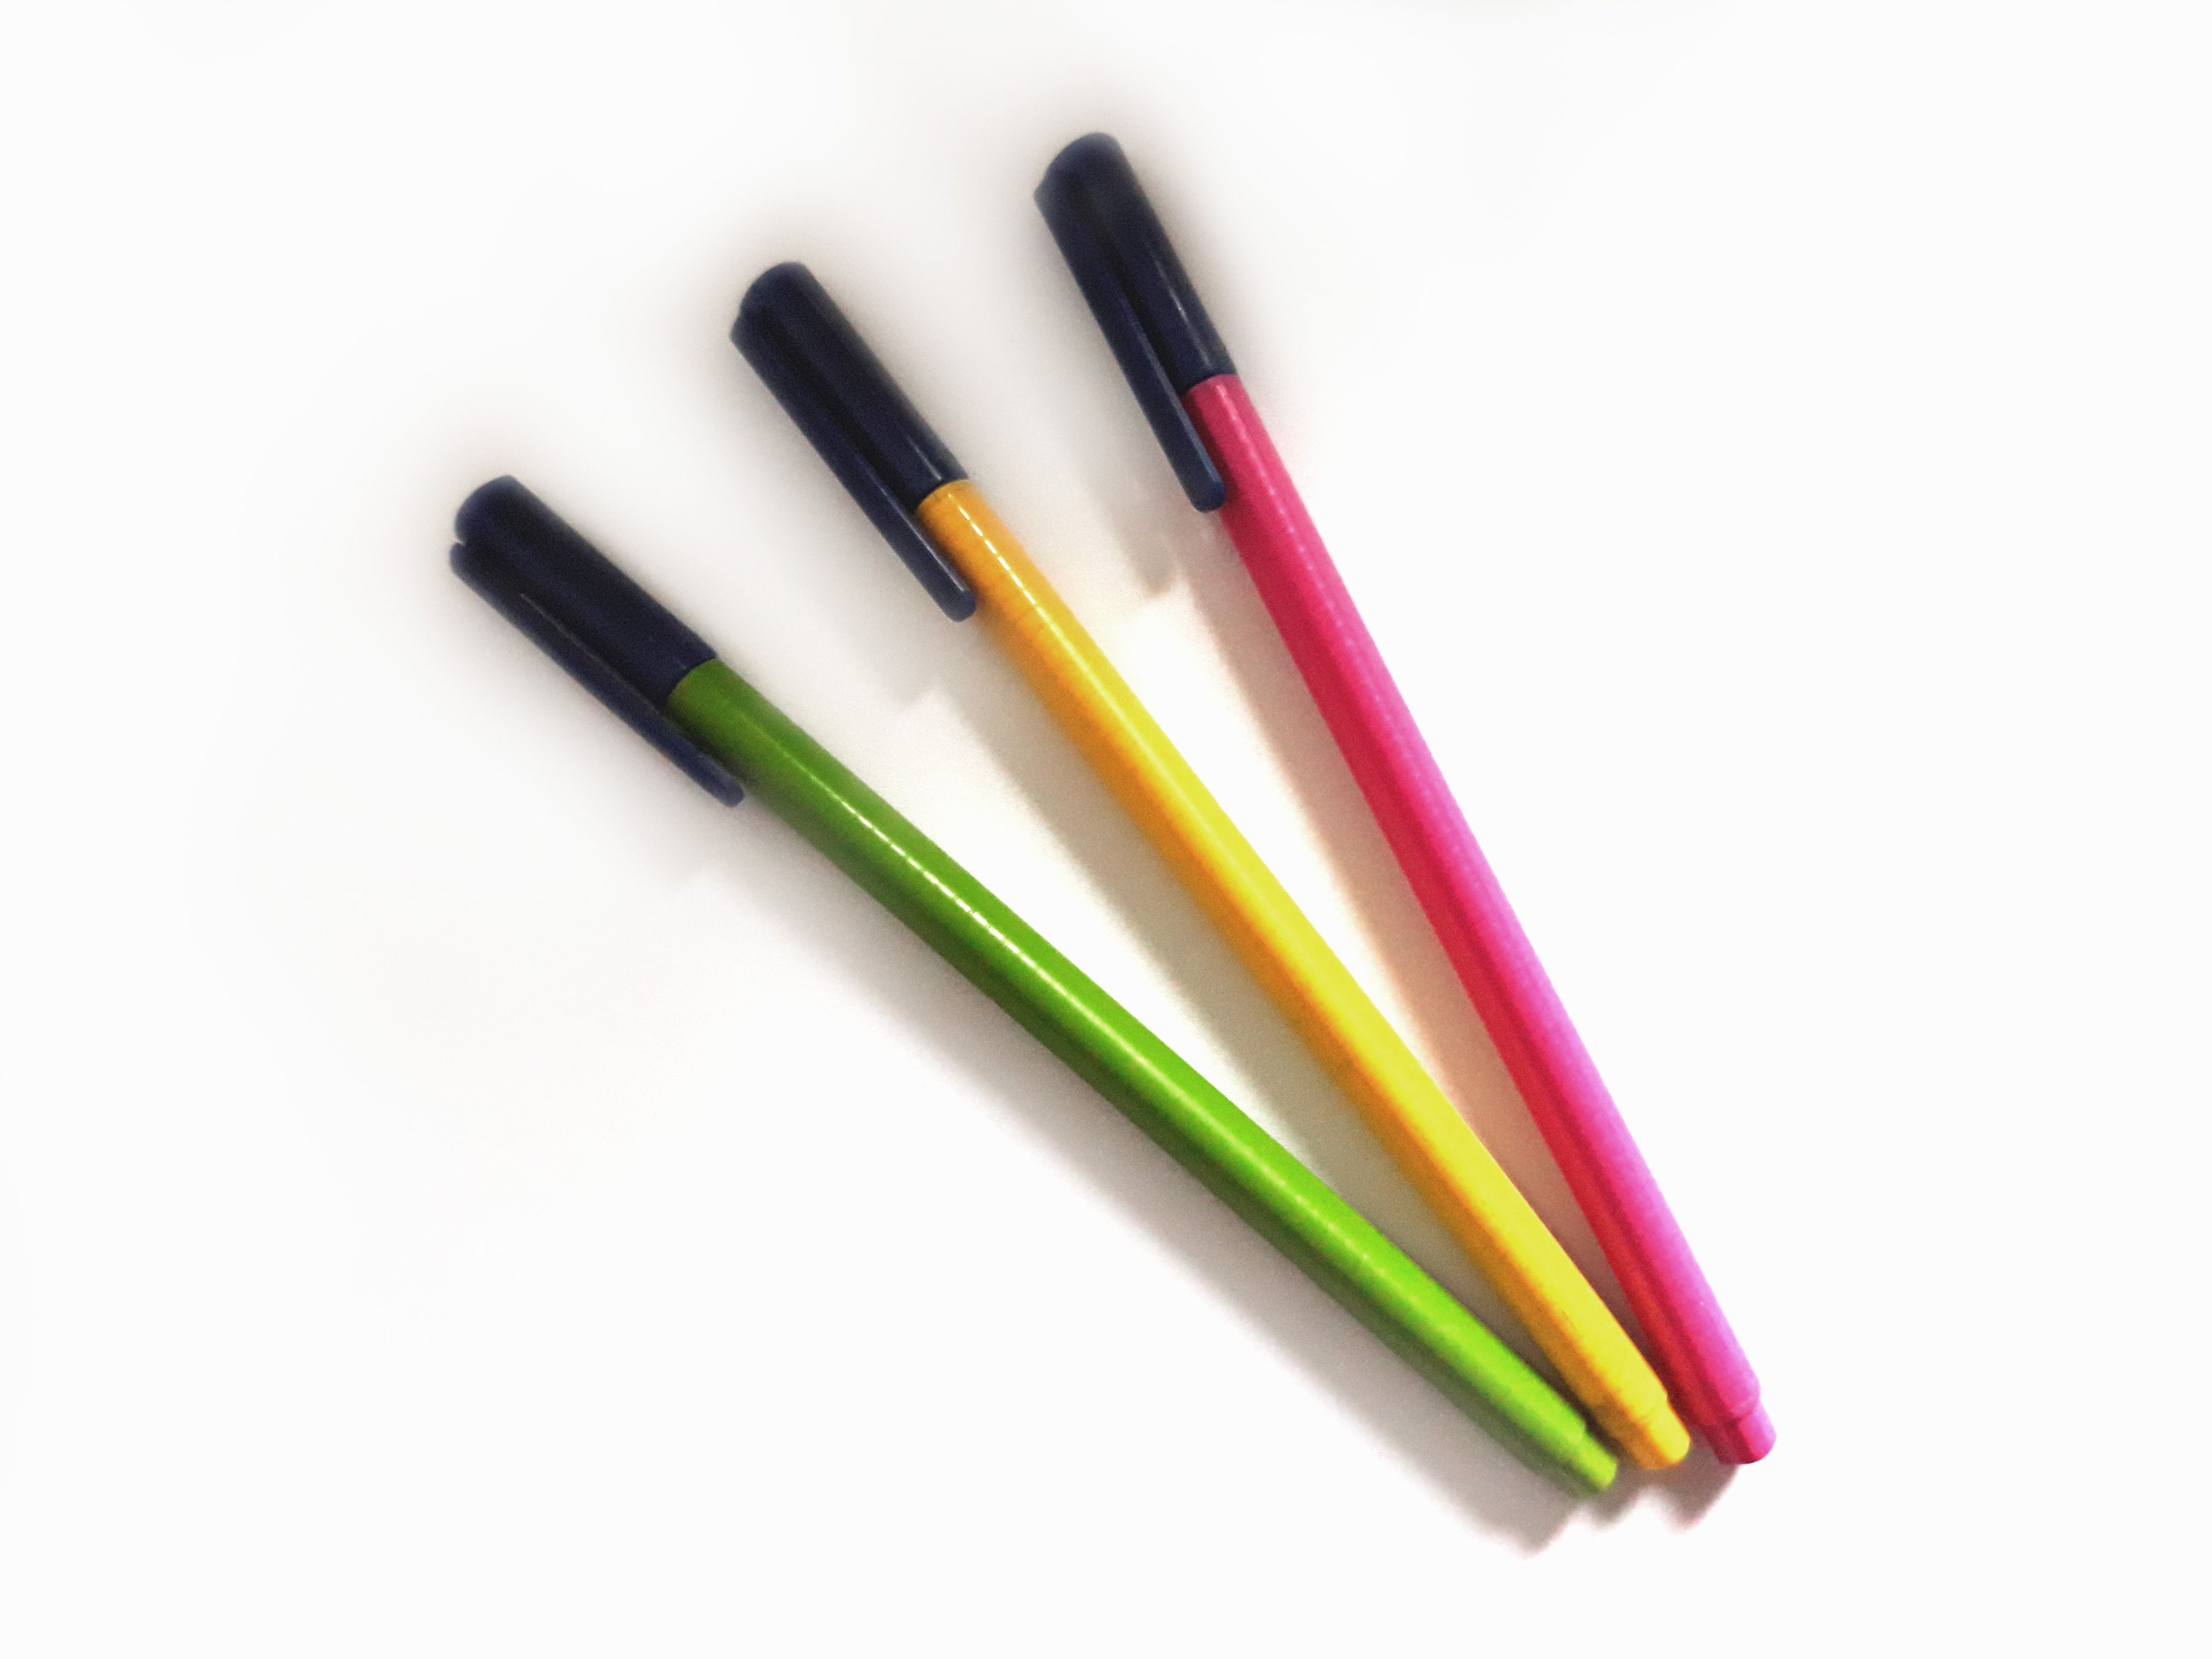
\includegraphics[width=5cm]{stift.jpg}
\caption*{Stifte}
}
\qquad
\begin{minipage}{5cm}
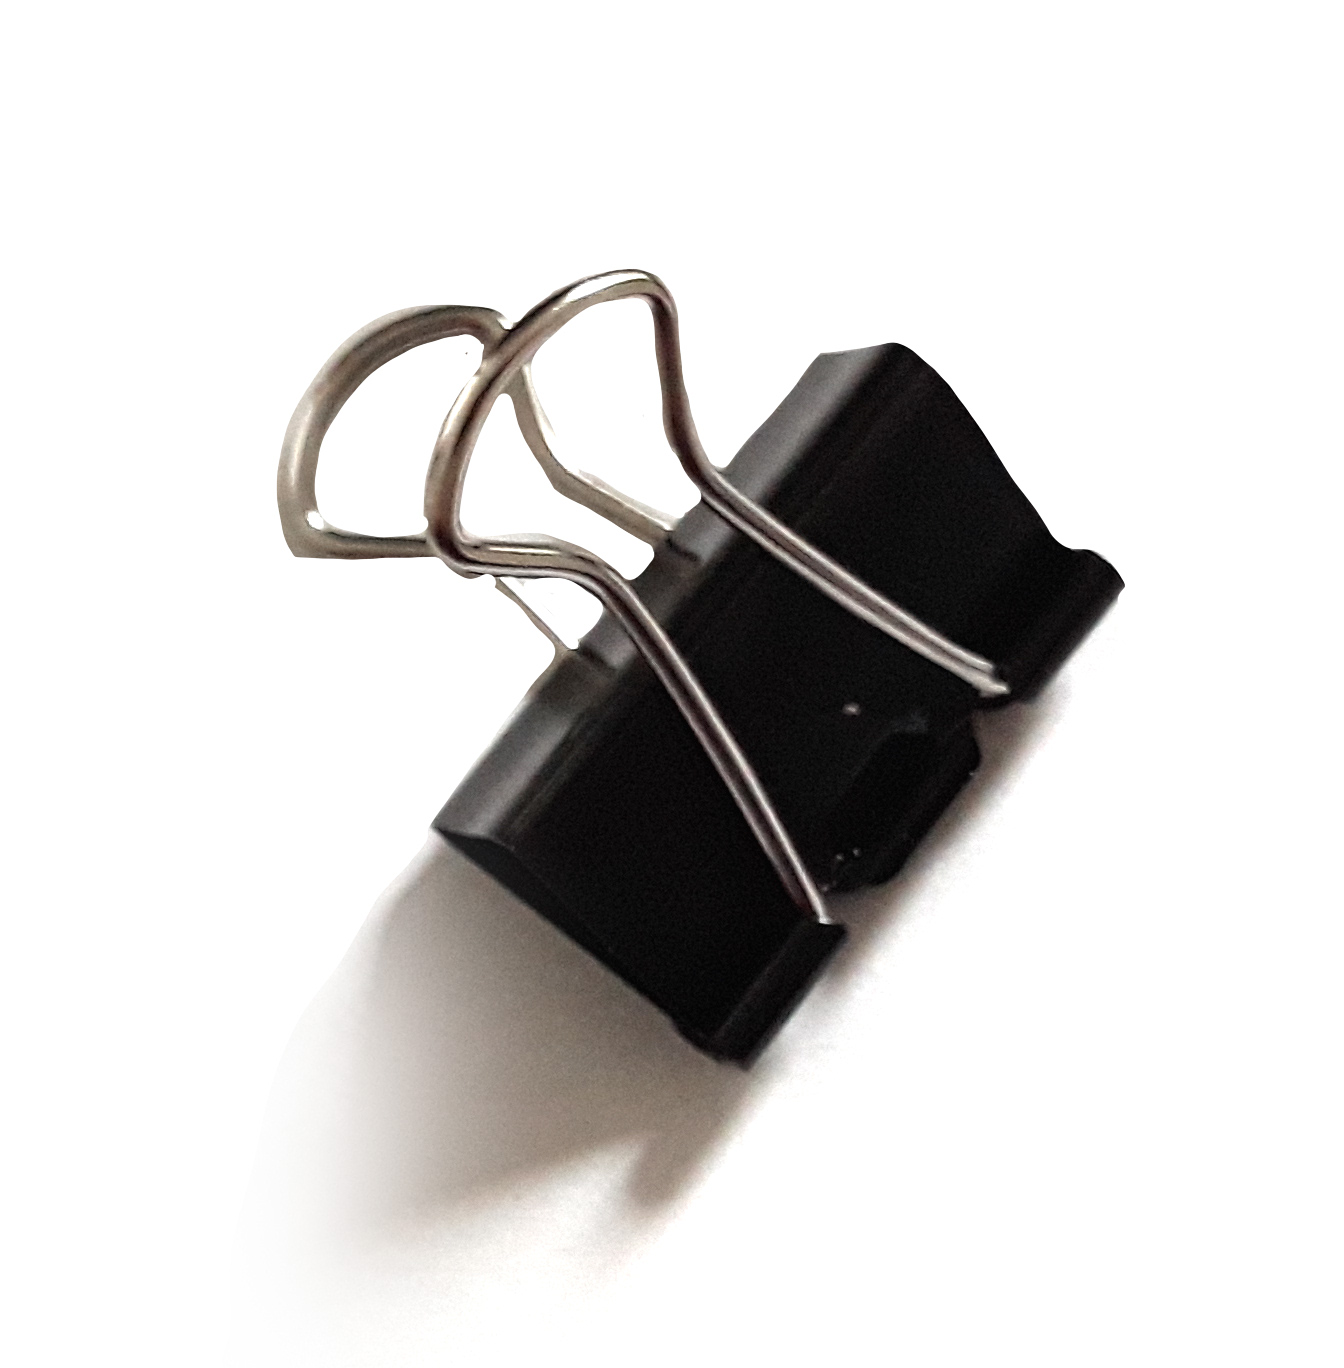
\includegraphics[width=5cm]{klammer.jpg}
\caption*{Klammer}
\end{minipage}
\end{figure}

\begin{figure}[h]
\centering
\parbox{5cm}{
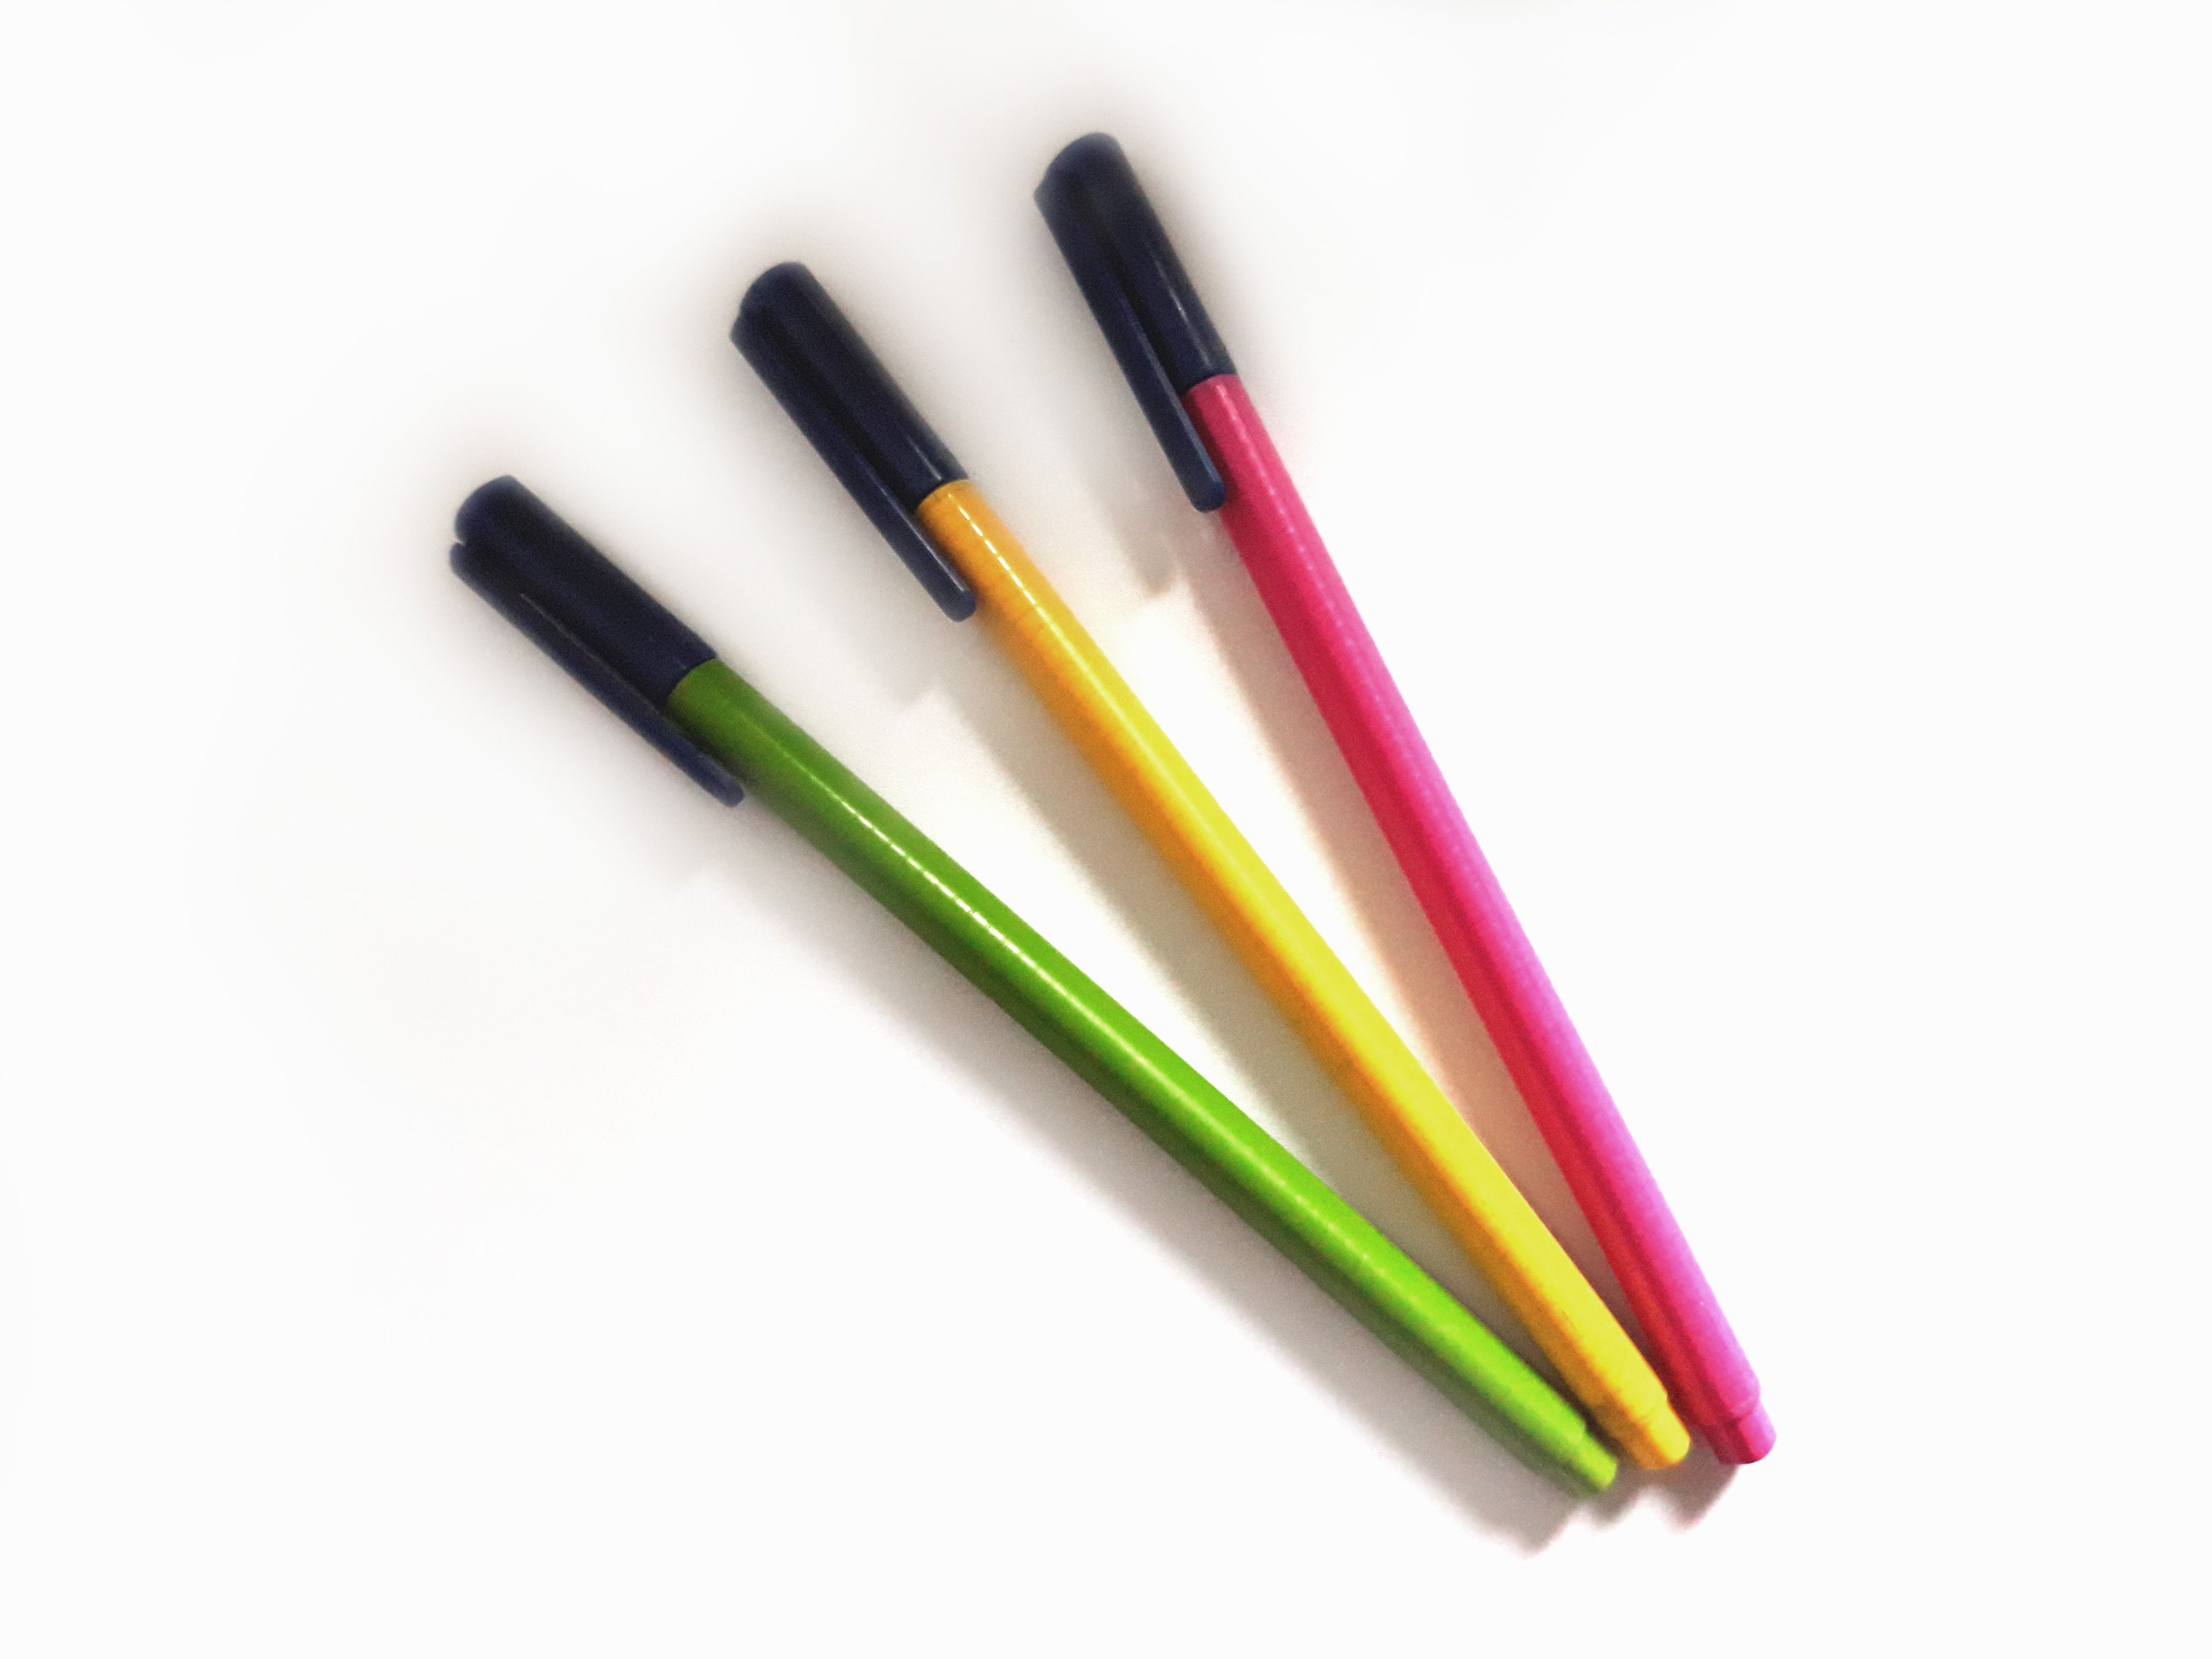
\includegraphics[width=5cm]{stift.jpg}
\caption*{Stifte}s
}
\hfill
\begin{minipage}{5cm}
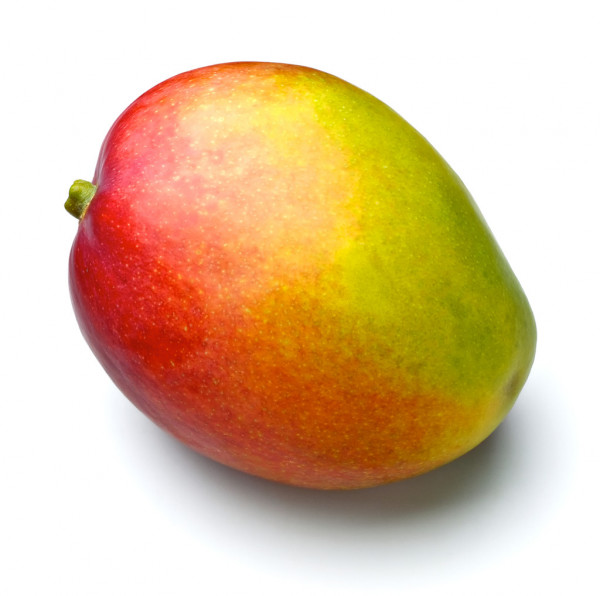
\includegraphics[width=5cm]{mango.jpg}
\caption*{Mango 2}
\end{minipage}
\end{figure}

\subsection{Materialien}

\subsubsection{Werkzeuge}
\begin{checklist}
    \item Heißklebepistole
    \item Schere / Teppichmesser

    \begin{checklist}
    \item[] Optional:
    \item Abisolierzange
    \item Lötkolben
    \end{checklist}
\end{checklist}

\subsubsection{Material}
\begin{checklist}
    \item RaspberryPi
    \item Bildschirm + HDMI-Kabel
    \item Maus
    \item Tastatur
    \item Zahnstocher
    \item Motoren
    \item Treiber
    \item Pappe
    \item Kabel
    \item Räder
    \item Klammern
    \item 4-AA-Batteriefach
    \item 4 AA Batterien
    \item Unterlage (Telefonbuch / Karton)
    \item X Female-Female Jumperkabel
    \item 1x Female-Male Jumperkabel
\end{checklist}


\subsection{Software}
Auf dem RaspberryPi sollte bereits ein funktionierendes \emph{Betriebssystem} installiert sein. Es bietet sich \emph{Raspberry Pi OS} (Raspbian) an. \\

Bei dem ursprünglichen Projekt wurde die Programmierumgebung \emph{Scratch} verwendet. Da diese die Ansteuerung von Motoren mit dem Raspberry Pi jedoch unnötig kompliziert macht, wurde hier auf die Verwendung der Programmiersprache \emph{Python} ausgewichen. Python bietet zwar keine grafische Programmieroberfläche (wie Scratch), ist jedoch, nach Meinung der Autoren, eine für alle Altersgruppen intuitive und mindestens genauso zugängliche Programmiermethode wie Scratch.\\

Vorkenntnisse über Python sind nicht zwingend notwendig!

\subsubsection{Script}
Zur Vorbereitung sollten einige Funktionalitäten innerhalb von Python eingebaut werden, welche die Verwendung bei der Kursdurchführung für die Kursteilnehmer erleichtern. Die Nachfolgenden Programme sollten vorbereitet werden.\\

Führen Sie folgende Schritte durch, sofern die genannten Ordner und Dateien nicht bereits vorhanden sind:\\

\schritt{1}{Legen Sie einen Projektordner an}{

  Legen Sie auf dem Desktop des Raspberry Pi einen neuen Ordner an und nennen Sie ihn \emph{Malroboter}.\\

}

\schritt{2}{Erstellen Sie zwei neue Dateien}{

  Erstellen Sie im Ordner Malroboter die folgenden Dateien:
  \begin{itemize}
  \item \emph{motorsteuerung.py}: Diese Datei dient der Übersetzung der bestehenden Funktionen und der Definitionen innerhalb des Projektes und wird i.d.R. nicht von den Kursteilnehmern verwendet.
  \item \emph{kurs.py}: Diese Datei soll dann von den Kursteilnehmern programmiert werden, hier wird z.B. die Geschwindigkeit der Motoren eingestellt.
  \end{itemize}


}

\vspace{\baselineskip}

\schritt{3}{Fügen Sie das Steuerungsprogramm ein}{

 Fügen Sie den folgenden Programmtext in die Datei \emph{motorsteuerung.py} ein:\\
  \indent \hinweis Sie finden die Programmdateien auch \href{https://www.github.com/latenighticecream/malroboter/Malroboter}{hier}\footnote[2]{https://www.github.com/latenighticecream/malroboter/Malroboter}.\\

}

\emph{motorsteuerung.py}\\
\lstinputlisting{Malroboter/motorsteuerung.py}
\vspace{\baselineskip}

\schritt{4}{Binden Sie das Steuerungsprogramm ein}{
Öffnen Sie die Datei \emph{kurs.py} und fügen sie den folgenden Programmtext ein:
\lstinputlisting{Malroboter/kurs.py}
}

